\section{Training on downscaled images}
\label{sec:practical}

\subsection{The measured $(\text{route}, \sigma)$ map}
\label{sec:verdict}
\label{sec:map}

The answer to the title question at our operating point is not a
corrected formula but a measured map at a stated resolution: the
curves both accounts were scored on carry the verdict, read per bin
against the safety statement of Eq.~\ref{eq:safe}
(Fig.~\ref{fig:verdict}; per-bin numbers in Appendix
Table~\ref{tab:debiasedmap}). Collected route by route --- \emph{safe}
meaning Eq.~\ref{eq:safe} holds at the stated margin, on the
\emph{per-example} object --- the map needs no table: $1024{\to}896$
(floor $0.02$--$0.04$) is \textbf{safe} on the interior window
$\sigma \in (0.5, 1)$, certified at margin $0.09$ simultaneous over
the seven window bins ($0.066$ pointwise; the strict
$\varepsilon = 0.02$ margin is not yet powered on the interior grid,
and powering it is a draw-count exercise, designated for the next
probe campaign); $1280{\to}1024$ (floor ${\approx}\,0$) is
\textbf{safe} from $\sigma \gtrsim 0.75$, and the synthetic
iso-severity grid $1280{\to}1120$ is safe with
$\sigmastar \approx 0.5$, as its ratio twin predicts (both
$1280$-tier reads on the pre-debiasing instrument;
\S\ref{sec:limitations}); $1024{\to}768$ and $896{\to}768$ (floors
$0.06$--$0.13$) have \emph{no certifiable window}; and any route to
$512$ (floor ${\approx}\,0.30$) is \emph{certifiably unsafe} in all
fifteen bins --- no noise level comes near certifying a $2\times$
downscale. Safety is a per-route boundary, jointly determined by
ratio (through $a_e$) and absolute target size (through $\Floor_e$);
neither alone predicts the ordering. Debiasing itself moved verdicts
in both directions, and the two revisions against the historical
record are part of the result: roughly half the $768$ route's
high-$\sigma$ plateau was estimator bias, softening ``unsafe at every
noise level'' to no-certifiable-window, while the $896$ endpoint
shows a small \emph{real} gap ($+0.034 \pm 0.011$) that
single-estimate variance had buried --- its safe window is the
interior, not the endpoint (Appendix Table~\ref{tab:rawendpoint}).

\paragraph{A corollary worth stating plainly.}
The safety of $1024{\to}896$ is an \emph{empirical smoothness statement
about this network's function across nearby token counts}, not an
information-theoretic statement about the data. There was no a priori
reason to expect a universal ratio invariant, and the spectral
account's deepest error is having promised one.

\paragraph{The map depends on the aggregation object.}
The aggregation operator is part of the estimand
(\S\ref{sec:estimand}, Appendix~\ref{app:notation}), and the two
objects genuinely disagree at high $\sigma$: pooled-arm probes (pool
size $4$) collapse the $1024{\to}896$ and $1024{\to}768$ excesses to
${\approx}\,0$ over the upper bins --- the batch-aggregate object SGD
follows is more forgiving here than the per-example read we publish
as the verdict. The coherent drift no batch size removes is bounded
only by an $a + b/B$ fit across pool sizes, the designated readout of
a debiased verdict grid at the shipped trainer's actual
batch$\times$accumulation operating point \textbf{[pending]}.

\subsection{$\sigma$-conditional training on the measured-safe route}
\label{sec:trainer}

We wire the one measured-safe corpus route into the LoRA trainer as an
opt-in path, exactly as measured, with no extrapolation beyond the map.
The intervention is deliberately small: three lines inside an otherwise
standard flow-matching step, and no change to the objective, the
optimizer, or the noise density (pseudocode in
Table~\ref{alg:sigmastep}).

\textbf{$\sigma$-first draw.} The trainer draws each batch's $\sigma$
\emph{before} fetching latents, from the unchanged training density
(demotion conditions on $\sigma$, not the reverse). When every sample
in the batch is above the gate ($\sigma > 0.5$), the native
$1024$-tier latent is swapped for a cached demoted-grid sibling
produced by the probe's own measured-safe recipe (pixel-space
downscale, VAE re-encode); everything downstream derives from the
swapped latent. Off-route images always train native, as does
validation. One honest asymmetry between the gate and the map must be
stated: the gate is one-sided ($\sigma > 0.5$) while certification
stops at $\sigma = 0.94$, and the endpoint carries a small real gap
($+0.042 \pm 0.011$). Since the expected gradient should vary
continuously in $\sigma$, that gap cannot be dismissed as a
measure-zero boundary point --- it implies a neighborhood, of
unmeasured width, over which some of it survives, and the tail
$\sigma \in (0.94, 1)$ is exactly the interval the verdict grid does
not resolve. Two facts bound the exposure meanwhile: the last
interior bin reads $+0.004 \pm 0.021$, and the exercise grid of
Table~\ref{tab:yardstick} trained \emph{with} the tail demoted and
still landed a factor $2$--$3$ inside the seed lottery, so any tail
effect is below that instrument's resolution at $480$ steps. A dense upper-tail sweep
($\sigma \in (0.9, 1)$ in four bins plus the endpoint, at higher draw
count) is designated to resolve the shape; until it lands, the
certified condition is $\sigma \in (0.5, 0.94]$, and the unbounded
gate should be read as the form we exercised, not the form the map
certifies.

\textbf{Banded rotary alignment, $\sigma$-gated.} Motivated by
\S\ref{sec:ourscored}, a frequency-selective alignment (YaRN-style
bands: full positional-interpolation stretch for rotary bands with few
rotations across the demoted extent, native spacing for high-frequency
bands, ramp between, thresholds scheduled by a sigmoid gate in $\sigma$
following \citealp{zhao2026sigma}) is applied on demoted forwards only.
Unlike uniform interpolation it is \emph{not} off-manifold in-window:
it passed both pre-registered legs, erasing the static variant's
low-$\sigma$ liability ($+0.064 \to +0.033 \pm 0.025$) while preserving
its high-$\sigma$ gains (paired $-0.05$ vs plain demotion at
$\sigma \ge 0.59$). It is a refinement candidate, not a gate-widener:
the gate stays $\sigma > 0.5$. Under bit-exact deterministic training
it adds no weight-space displacement over the demotion arm it refines
(base$\leftrightarrow$refined $0.319$ vs base$\leftrightarrow$demoted
$0.320$; without determinism a twin-run chaos floor of $0.41$ would
swamp this read).

\textbf{Cost accounting.} With ${\sim}50\%$ of draws above the gate and
the demoted forward at ${\sim}0.72\times$ tokens, the fixed-step epoch
cost is ${\approx}\,0.86$, a \emph{projected ceiling} of ${\sim}14\%$
wall-clock on our corpus ($96\%$ of records are on the safe route),
scaling with high-tier content. On the fixed-step exercise grid below
the realized saving is $-15.1\%$ forward FLOPs (exact operator-level
counts over each run's realized token histogram) and $-14.6\%$
wall-clock ($n{=}3$ seed means on two single-artist corpora; wall
tracks FLOPs ${\approx}\,1{:}1$): the projection is achieved. The claim
is wall-clock at fixed steps, not ``more steps in the same time.''

\begin{table}[t]
\begin{minipage}[t]{0.615\linewidth}
\caption{Weight-space footprint vs.\ the seed lottery: cosine between
adapter endpoints, $\cos(\Delta W_{\text{arm}}, \Delta W_{\text{native}})$
at matched training seed, mean $\pm$ seed spread (SD over the three
matched-seed pairs; the three seed pairs for the yardstick row), on two
single-artist corpora ($60$/$15$ training images). The yardstick row is
the same cosine between native endpoints that differ \emph{only} in
training seed (arm-independent: the shipped arm's cross-seed values
coincide with it within $.006$). An arm reading above the yardstick
displaces the endpoint \emph{less} than a seed change does. Training is
bit-exact deterministic --- an identical retrain reads $1.000$ --- so
the table reads caused displacement, not run-to-run chaos. \emph{late}:
demotion restricted to the last $75\%$ of steps; the stacked row adds a
second certified route ($1024{\to}768$ on $0.65{<}\sigma{<}0.95$, last
$50\%$) on top of \emph{late}. \textbf{Bold}: the late-scheduled arms
--- the closest endpoints; the stacked row adds strictly deeper
substitutions at no endpoint cost, an ordering set by placement that a
per-step spectral account cannot produce.}
\label{tab:yardstick}
\centering
\footnotesize
\setlength{\tabcolsep}{3pt}
\begin{tabular}{@{}lcc@{}}
\toprule
arm (vs.\ native, matched seed) & corpus A & corpus B \\
\midrule
native, cross-seed (yardstick) & $0.121 \pm .007$ & $0.199 \pm .003$ \\
\midrule
$896$, $\sigma{>}0.5$, aligned & $0.365 \pm .020$ & $0.432 \pm .026$ \\
\quad + late & $\mathbf{0.753 \pm .019}$ & $\mathbf{0.770 \pm .009}$ \\
\quad + late, stacked $768$ & $\mathbf{0.753 \pm .017}$ & $\mathbf{0.771 \pm .009}$ \\
$896$, every $\sigma$ & $0.183 \pm .009$ & $0.236 \pm .009$ \\
\bottomrule
\end{tabular}
\end{minipage}\hfill
\begin{minipage}[t]{0.355\linewidth}
\caption{The shipped step, in full. Lines 3--5 (colored) are the
entire change: the gate $\sigmastar{=}0.5$ and the route are read off
the measured map (\S\ref{sec:verdict}), line 5 is the optional
refinement, and lines 1--2 are only a reordering of a standard step
--- $\sigma$ is drawn before the latent is fetched.}
\label{alg:sigmastep}
\centering
\footnotesize
\setlength{\tabcolsep}{2pt}
\begin{tabular}{@{}>{\ttfamily}r@{~}>{\ttfamily}l@{}}
\toprule
\multicolumn{2}{@{}l@{}}{\textbf{one LoRA training step}} \\
\midrule
1 & $\sigma \sim p_{\mathrm{train}}$ \\
2 & $x \leftarrow$ native latent of $y$ \\
\addedline{3} & \addedline{if $\sigma > \sigmastar$ and $y$ on-route:} \\
\addedline{4} & \addedline{\quad $x \leftarrow$ demoted latent of $y$} \\
\addedline{5} & \addedline{\quad rotary $\leftarrow$ banded$(\sigma)$} \\
6 & $\epsilon \sim \mathcal{N}(0, I)$ at shape$(x)$ \\
7 & $z \leftarrow (1{-}\sigma)x + \sigma\epsilon$ \\
8 & $v \leftarrow \epsilon - x$ \\
9 & step on $\|\hat v_\theta(z, \sigma, c) - v\|^2$ \\
\bottomrule
\end{tabular}
\end{minipage}
\end{table}

\begin{figure}[t]
\centering
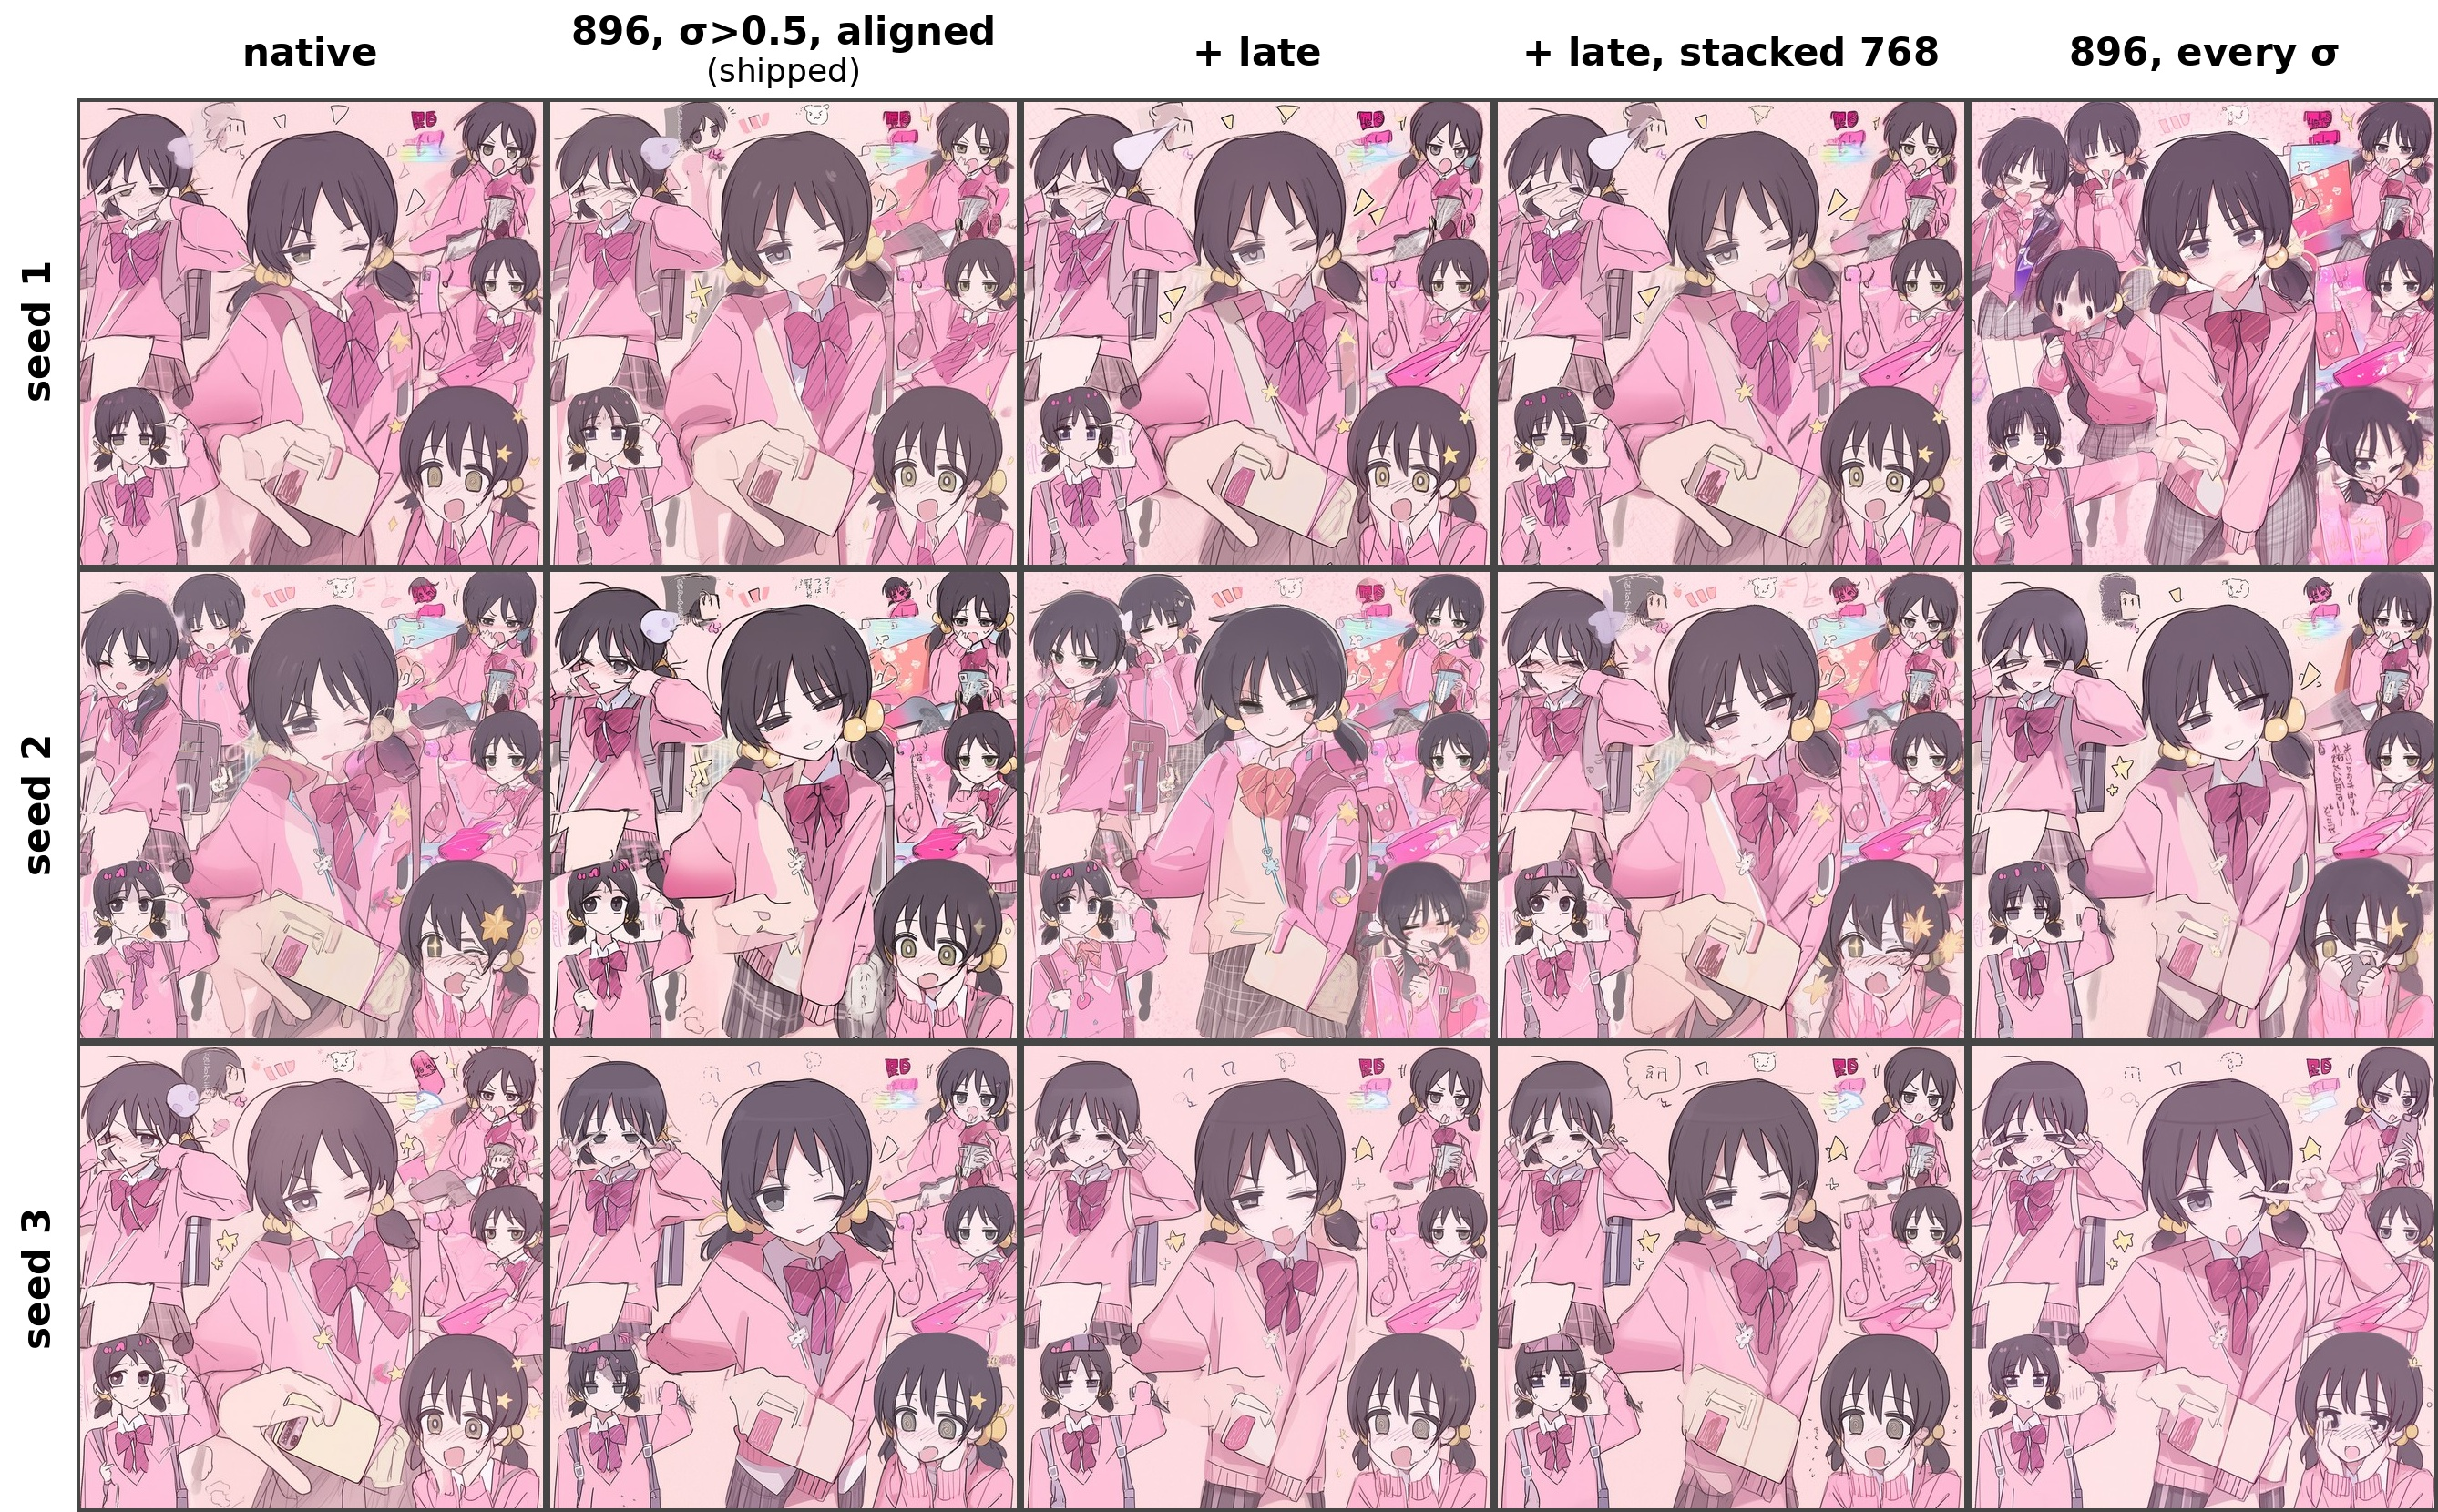
\includegraphics[width=\linewidth]{figs/kaai_yuki_arms_grid.jpg}
\caption{Visual counterpart to Table~\ref{tab:yardstick}: matched
(prompt, noise-seed) renders from each arm's endpoint on a corpus-B
display prompt, $20$ steps; columns are the table's arms, rows the
three training seeds. Moving along a row (arms, seed fixed) changes
the render on the same visual order as moving down a column (seed
lottery, arm fixed); the gate-removed arm (rightmost) drifts the
most, matching its eroded margin in Table~\ref{tab:yardstick}.}
\label{fig:kaaiyuki}
\end{figure}

\textbf{Weight-space endpoint footprint.} A fixed-step exercise grid
(gated, scheduled, and gate-removed arms $\times$ $3$ training seeds
$\times$ $2$ single-artist corpora, $480$ optimizer steps each,
bit-exact deterministic paired-RNG so every arm sees identical draws)
compares the trained adapters directly in weight space.
Table~\ref{tab:yardstick} reads the cosine between each arm's endpoint
$\Delta W$ and its matched-seed native twin's, judged against a
seed-noise yardstick: the same cosine between native endpoints that
differ only in training seed. Determinism makes the read exact --- an
identical retrain reproduces its twin at $1.000$ --- and the yardstick
is tight, so the margins are many seed-spreads wide. Every arm lands
above the yardstick: even demoting \emph{all} $480$ steps displaces the
endpoint less than changing the training seed, and the shipped gate
sits a factor $2$--$3$ above it ($0.365$ vs $0.121$; $0.432$ vs
$0.199$). The ordering, however, is set by \emph{placement}, not by
per-step severity: protecting the first quarter of training doubles the
closeness ($0.365 \to 0.753$) --- consistent with early subspace
selection in a from-zero adapter --- and stacking a strictly deeper
certified $768$ route onto the late rule is endpoint-free ($0.753$,
$0.771$), although the spectral account of \S\ref{sec:ourscored} prices
every $768$ substitution as more severe than $896$. A per-step account
is placement-blind by construction; the endpoint statistic resolves
what it cannot: \emph{when} a demoted step happens dominates \emph{how
deep} it goes, provided the route stays inside the certified window.
Removing the $\sigma$-gate erodes the margin toward the lottery radius
($0.183$; $0.236$). Weight-space proximity is a footprint statement,
not a quality statement: sample-level orderings need not track it, and
generation-quality non-inferiority at production scale remains the
stated open gate (\S\ref{sec:limitations}).

\section{Limitations}
\label{sec:limitations}

\textbf{One model family, one operating point.} All gradient probes ran
on one DiT (Anima) with one adapter checkpoint trained at native tiers.
A mixed-resolution-trained adapter might equalize (or widen) its own
gradients; probing such a checkpoint is the designated bound on how far
the map generalizes, as is re-probing $1280{\to}1024$ after fine-tuning
at the 1280 tier. The probe pool's relationship to the adapter's own
fine-tune set was measured rather than conceded: a controlled
$2{\times}2$ factorial (two LoRAs trained on opposite style clusters
under frozen membership manifests, probed on both) replicates the map's
shape on both checkpoints with the adapter$\times$probe-style
interaction below instrument resolution, while the absolute
redraw-floor level is checkpoint-dependent (Appendix~\ref{app:e7}).

\textbf{Gradient-level, not end-task.} The map is built from
accumulated per-step gradients; integration over an optimizer
trajectory is addressed by the exercise grid's weight-space read at
$480$ steps rather than production scale, and the
generation-quality (CMMD, \citealp{jayasumana2024cmmd}) gate remains
open: the exercise grid's first scoring pass could not separate even
the off-map control from native at this scale, so we read no quality
verdict from it.

\textbf{Account resolution and domain.} The account predicts held-out
routes at ${\sim}0.07$--$0.09$ RMSE, not within $\epsstar$; its
$A(\mathrm{ratio})$ governor rests on two distinct ratio values; the
reduction's domain excludes the $768$ mid-$\sigma$ window, whose
mechanism the vector-resolved probe has measured (negative
interference) but which the two-term form still does not predict; the
floor law's functional form is unidentified at our operating points;
and the band-counting sketch for $\mathrm{RoPE}_e$/$\mathrm{Resid}_e$
is calibrated, not derived. The graph-floor reading of the endpoint is
also estimand-specific: the target-mediated perturbation is real at the
vector level and lands parallel to the native gradient
(Appendix~\ref{app:instrument}), so a magnitude-sensitive estimand ---
an un-normalized optimizer, say --- could apportion the endpoint gap
differently than the angular read does.

\textbf{Instrument resolution and coverage.} ``Safe'' is one-sided
non-inferiority against a fixed margin ($\varepsilon = 0.02$ strict;
the interior window currently certifies at $0.056$--$0.07$), with the
certification resolution ($\epsstar = 0.03$--$0.08$ per bin;
${\approx}\,0.01$--$0.02$ at the endpoint sweeps) setting the power
available, not the margin. True gaps below $\epsstar$ are undetectable
by construction, $\sigmastar$ boundaries are localized only to a bin,
and every ``no certifiable window'' claim is $(N, D)$-relative: a
larger campaign could certify (or refute) the $768$ high-$\sigma$
window at the strict margin. The upper tail $\sigma \in (0.94, 1)$ of
the safe route is unmeasured between the last interior bin and the
endpoint's real gap; the designated dense sweep (\S\ref{sec:trainer})
closes it. Verdict stability under the per-image trim rule of
\S\ref{sec:instrument} has not been separately audited. The
debiasing campaign covered the corpus verdict grid; the $1280$-tier
iso-severity, $896$-tier transfer, depth-split, and PI-intervention
probes remain pre-debiasing reads, and the $1280$-tier curves enter the
held-out validation on that basis.

\textbf{Scope.} Adapter (LoRA) gradients on a frozen backbone; full
fine-tuning may differ. Pixel-space demotion only (latent-space
downsampling was not tested here; SwD found it inferior). The
$\sigma$-gated banded-alignment parameters were taken from one shot at
pre-registered values, not searched.

\section{Conclusion}
\label{sec:conclusion}

When does training on downscaled images yield the same gradient
direction? Not
when the noise has masked the frequencies the coarse grid loses. That
spectral answer was advanced by prior work for inference-time
substitution and had not previously been confronted with the training
gradient; transported to the training question it is a model of only
one part of one branch of what demotion perturbs, and the measurements
reject it at every point of structural divergence --- the mildest
route's crossover sits at $3.5\times$ the equal-power prediction, no
tolerance reproduces the map, its one free parameter is inert at the
curve level, and a $2\times$-downscaled latent certifies at no noise
level, because the network function itself is
grid-calibrated: partly through its positional coordinate system,
partly through an irreducible dependence of the computation on token
count.

The measured answer has two conditions, matching the two terms of our
account: the target grid must be large enough in \emph{absolute token
count} that its graph floor sits below certification resolution, and the
noise level must exceed a per-route boundary where the ratio-governed
data term dies. On our model that means $1024{\to}896$ on
$\sigma \in (0.5, 0.94]$ (the upper tail toward the endpoint's small
real gap still unresolved) and $1280{\to}1024$ at
$\sigma \gtrsim 0.75$, and a $2\times$ downscale at no noise level. The answer is predictive, not
merely descriptive: head to head on the same curves the account
predicts held-out routes at ${\sim}0.07$--$0.09$ RMSE against the
spectral family's $0.147$--$0.355$, beating an oracle fit on the
held-out data itself on one route. Getting there required treating the
question as a metrology problem: naive finite-draw estimation
manufactures exactly the token-count-ordered floor signature under
test, half the intermediate route's raw floor was estimator bias, and
our own headline claims were re-derived, and in one case softened,
under the correction. On the one route our corpus makes safe, the
trainer realizes the map's projected ceiling ($-14.6\%$ wall-clock at
fixed steps) with a weight-space endpoint footprint a factor $2$--$3$
inside the seed lottery --- rising to cosine $0.75$ against the native
endpoint when demotion is late-scheduled;
quality non-inferiority at production scale remains the open gate. We
offer the account and its instrument as the cheap, general test that
any future ``train part of the time at lower resolution'' proposal
should pass before it is believed --- and without the debiasing, that
test manufactures the very effect it looks for.

\subsubsection*{Reproducibility statement}
The probe scripts (\texttt{run\_sigma\_probe.py}, including the
\texttt{--self\_floor} and \texttt{--draw\_sweep} debiasing modes;
\texttt{run\_prior\_distance.py}, \texttt{rapsd.py},
\texttt{compare\_ckpt\_dw.py}), the held-out validation and refit
analyses (\texttt{e5\_holdout.py}, \texttt{e5\_refit.py},
\texttt{e83\_bridge.py}), the trainer wiring
(\texttt{--sigma\_lowres}), and the frozen pre-registration documents
are in the public repository at
\url{https://github.com/sorryhyun/anima_lora} (project line
\texttt{project/sigma\_lowres/}), together with the debiased verdict
runs' complete per-image records. The earlier raw-instrument archives
are excluded by the repository's results ignore rule and will be
published as a companion tarball \textbf{[pending]}; until then those
numbers are reproducible from the scripts but their original records
are not public. Paired training runs use a \texttt{--deterministic}
mode verified bit-identical across twin runs; finite-draw cosines are
kernel-path-sensitive, so all cosine pairings are computed within a
single run (Appendix~\ref{app:instrument}).
